%%%%%%%%%%%%%%%%%%%%%%%%%%%%%%%%%%%%%%%%%%%%%%%%%%%%%%%%%%%%%%%%%%%%%%%%%%
%
%    JWST_sci_template.tex  (use only for JWST General Observer and Archival Research proposals)
%
%
%
%Z    JAMES WEBB SPACE TELESCOPE
%    OBSERVING PROPOSAL TEMPLATE
%    FOR CYCLE 1 (2017)
%
%    Version 1.0 September 2017.
%
%    Guidelines and assistance
%    =========================
%     Cycle 1 Announcement Web Page:
%
%         https://jwst-docs.stsci.edu/display/JSP/JWST+Cycle+1+Proposal+Opportunities
%
%    Please contact the JWST Help Desk if you need assistance with any
%    aspect of your proposal:
%    	    http://jwsthelp.stsci.edu
%
%
%
%%%%%%%%%%%%%%%%%%%%%%%%%%%%%%%%%%%%%%%%%%%%%%%%%%%%%%%%%%%%%%%%%%%%%%%%%%%

% The template begins here. Please do not modify the font size from 12 point.

\documentclass[12pt]{article}
\usepackage{jwstproposaltemplate}
\usepackage{hyperref}
\usepackage{graphicx}
\usepackage{floatrow}
\usepackage{sidecap}
\usepackage{wrapfig}
\usepackage{soul}
\sidecaptionvpos{figure}{t}


\usepackage{caption}
\captionsetup[figure]{labelfont=bf, font=footnotesize}
\captionsetup[table]{labelfont=bf, font=footnotesize}

\usepackage{natbib}
\bibliographystyle{mnras}

\setlength{\textfloatsep}{5pt}
\usepackage{color}

\newcommand{\todo}[1]{\textbf{**TODO: \textcolor{red}{#1}**}}


\begin{document}

%   1. SCIENTIFIC JUSTIFICATION
%       (see https://jwst-docs.stsci.edu/jwst-opportunities-and-policies/jwst-call-for-proposals-for-cycle-1/jwst-cycle-1-proposal-preparation)
%
%

\clearpage

\justification          % Do not delete this command.

\textbf{We propose PUPPIES - the Public Ultradeep Pure Parallel Imaging Exploration Survey - a treasury pure parallel NIRCam public imaging program. PUPPIES will exploit the longest pure parallel opportunities to build $\sim 150\ {\rm arcmin^2}$ of deep (F200W$=29.2-29.6$, 5$\sigma$ point-source) multi-band imaging. PUPPIES will probe an area $1-2\times$ larger than the Cosmic Evolution Early Release Science Survey (CEERS) but $0.2-0.6$ mag deeper. While focused on exploring faint sources in the distant Universe, PUPPIES will enable a large amount of legacy science ranging from probing the population of low-mass stars and sub-stellar objects in the Milky Way to building a coherent picture of the assembly of stellar mass over much of the Universe's history.} 

% As such, \emph{Webb}'s capability will reveal how the first galaxies assembled, the nature of the sources that re-ionised the Universe, and how the diverse galaxy population we can study at $z \sim 3-6$ was established at higher redshifts.  We can observe galaxies up to $z \sim 7$ with Hubble, but we know from these observations that the first epochs of galaxy formation are several 100 Myrs earlier.  Therefore, \emph{Webb} has an excellent chance of seeing the very first epochs of galaxy formation.

%The past near-decade of wide and deep surveys with the {\it Hubble Space Telescope’s} ({\it HST}) Wide Field Camera 3 (WFC3) has begun the process of exploration of this key epoch in the Universe’s history.  

%Wide and deep surveys with WFC3 over the enabled the construction of the first large samples of galaxies at $z>7$.  

% This is an issue that will necessarily receive intense attention with \emph{Webb} from both GTO and GO observations.  Because this problem is observationally so difficult, but of vast importance, it will require innovative strategies and multiple data collecting methods.  We do not know if $z > 9$ galaxies will be a population of plentiful low mass ones, or less common high-mass galaxies.  Because of this, several different observing strategies are needed to fully explore this early epoch.

\noindent\textcolor[RGB]{160,160,160}{\rule{\linewidth}{0.2pt}}

The study of the first stars and galaxies (first light) is one of the scientific cornerstones of the \emph{Webb Telescope} and is built on the legacy established by the \emph{Hubble Space Telescope}. \emph{Hubble} spent thousands of orbits over three decades to constrain the evolution/formation of galaxies, which it can observe from when the universe was 500 Myr old until today.  This includes large dedicated projects such as the Hubble Ultra Deep Field (HUDF; \citealt{Beckwith2006, Bouwens2010, Dunlop2013}), the Cosmic Assembly Near-Infrared Deep Extragalactic Legacy Survey (CANDELS; \citealt{Grogin2011, Koekemoer2011}), and the Hubble Frontier Fields \citep{Lotz2017}. While these have led to significant insight into early galaxy formation  at redshifts $z \sim 6-8$ we have not yet reached the first epoch of galaxies, due to the \emph{Hubble}'s limited sensitivity and wavelength coverage. Little is therefore known concerning the galaxy population at $z > 9$ beyond the discovery of a few candidate galaxies (REFERENCES).  

In its earliest cycles \emph{Webb} will make progress in exploring the $z>9$ Universe through deep near-IR imaging. This enables the identification of individual galaxies and the measurement of many of their key properties including star formation rates, stellar masses, and dust attenuation. Through large tiered surveys \emph{Webb} will ultimately constrain the population demographics providing the essential observations to constrain galaxy formation models. Once identified, \emph{Webb}'s spectroscopic capabilities will be turned on these early galaxies yielding detailed constraints on their star formation and metal enrichment histories.

Planned GTO/ERS programs, in particular the Cosmic Evolution Early Release Survey (CEERS), the Webb Medium Deep Fields (WMDF), and the JWST Advanced Deep Survey (JADES), will begin the process of obtaining these constraints through multi-band NIRCam imaging. While immediately public, CEERS will probe a relatively modest $\sim 100\ {\rm arcmin^{2}}$ reaching just shy of F200W$=29$ ($M_{1500}\approx -18.5$ at $z=10$). Thus while CEERS will provide our first glimpse of the $z>9$ galaxy population it will yield poor constraints on the UV luminosity function. This is particularly true of the faint galaxy population, now well established to provide the bulk of the photons responsible for reionisation (Robertson et al.\ 2019; Finkelstein et al.\ 2019). On the other hand while JADES will  yield large numbers of $z > 9$ sources it surveys only a pair of contiguous fields leaving it susceptible to cosmic variance. Furthermore, JADES observations will not be immediately public, with the bulk of observations not publicly available until at least $2-3$ years after launch. 

One way to efficiently overcome these issues is with a pure parallel program. Like \emph{Hubble} before it, \emph{Webb} has the capability to use a second instrument in parallel to the prime observations. This allows us to obtain deep data across many independent locations on the sky virtually for free, critical for minimising cosmic variance. \emph{Hubble} pure parallel programs including HIPPIES \citep{Yan2011} and BoRG \citep{Trenti2011} were instrumental to providing constraints on the bright-end of the high-redshift $z>6$ luminosity function. Unlike \emph{Hubble} however, \emph{Webb} should have a large number ($>50$) of opportunities enabling the acquisition of deep (F200W$>29$, $5\sigma$ point-source) multi-band (4 or 6 filter) NIRCam imaging. 

\vspace{2mm}
\noindent
Hence we propose to exploit the deepest parallel opportunities to obtain F200W$=29-30$ ($5\sigma$ point-source) public imaging over an area $1-2\times$ larger than CEERS. This program - the \textbf{Public Ultradeep Pure Parallel Imaging Exploration Survey (PUPPIES)} - will tackle a range of science goals, with a strong focus on the $z>9$ Universe. Our primary objectives include: identifying $\sim 100$ galaxies at $z>9$: more than $3\times$ ($5\times$) the number expected in CEERS at $z>9$ ($z>11$); placing meaningful constraints on the faint-end of the $9<z<11$ luminosity function; and studying properties such as: star formation rates, stellar populations, dust attenuation, structure, and sizes and the correlations of these quantities. These are all important features for solving the very early formation of galaxies. In this respect PUPPIES will be a public data-set to complement GTO imaging programs for a full accounting of the $z > 9$ galaxy population and to test ideas and models concerning the formation of the first galaxies which need good statistics from low shot noise and sampling across luminosities. Beyond these primary objectives, PUPPIES will have tremendous legacy value enabling the answer of multiple open questions in both galactic and extragalactic astronomy. To aid in harnessing the tremendous legacy potential of PUPPIES we will rapidly release high-level data products, including reduced imaging, source catalogues, and catalogues with redshifts and physical properties from SED fitting.  


\subsection*{\bf \underline{Constraining the faint-end of the UV luminosity function at $z > 9$}}\label{sec:UVLF}


% Among the discoveries made with these data to date include: 1) A faint-end UV luminosity function slope which steepens at $z>4$, but a bright-end with less evolution (e.g., \citealt{Bouwens2015, Finkelstein2015}); 2) The abundance of galaxies from lensing studies (e.g., \citealt{Atek2015, Livermore2017}) implying that galaxies produce enough photons to complete reionization by $z\sim$ 6 (e.g., \citealt{Duncan2015, Robertson2015}); 3) Bright/massive galaxies appear modestly dusty, showing an early onset of chemical enrichment, with no signs of Pop III star colors (e.g., \citealt{Finkelstein2012, Bouwens2014, Bhatawdekar2020}), and 4) Some bright/massive galaxies exist out to at least $z \sim$ 10 (e.g., \citealt{Oesch2016, Salmon2018}) showing that potentially significant numbers of galaxies are waiting to be discovered at this early epoch of galaxy formation.


A primary goal for \emph{Webb} is placing constraints on the UV luminosity function across the epoch of re-ionization $6<z<12$, particularly at $z>9$ where existing constraints from \emph{Hubble} are based on only a handful of candidates.

The observed rest-frame ultraviolet (UV) luminosity function is the key observational diagnostic of the early galaxy formation. Many different physical processes determine and influence the formation and early evolution of the first galaxies, and thus the corresponding emergence of UV light. The gas density, processes of cooling, production of metals and dust, feedback processes and the role of magnetic fields all play a role. As demonstrated in Fig. \ref{fig:models} predictions of the formation of the first galaxies vary significantly depending on assumptions on these properties went into the models: despite good agreement at $z<8$ by $z=9$  predicted luminosity functions have diverged. Reproducing the observed luminosity function with plausible models is then a powerful approach for understanding the role of these processes in the early Universe.

 \begin{figure}[h!]
    \centering
    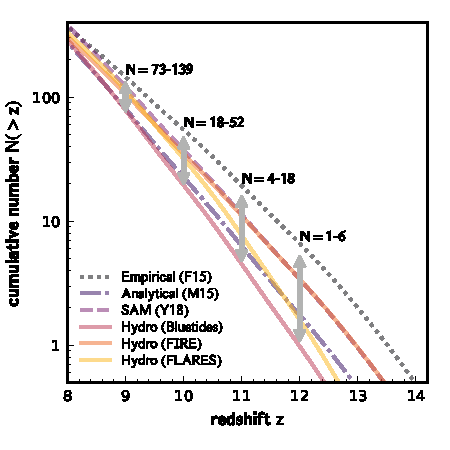
\includegraphics[width=0.49\textwidth]{figs/CN_models.pdf}
    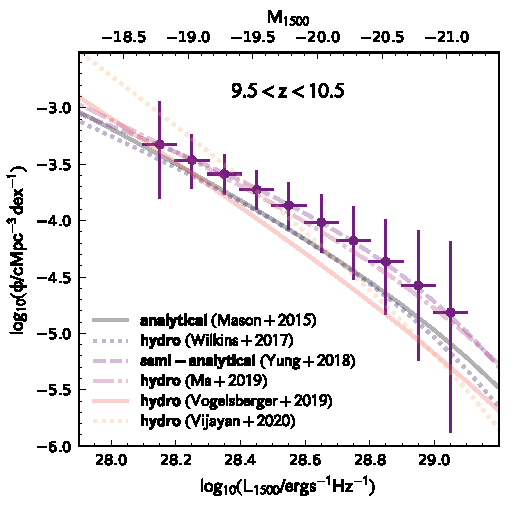
\includegraphics[width=0.49\textwidth]{figs/LF_models_10.pdf}
    \vspace{-5mm}
    \caption{\emph{\underline{Left:}} The cumulative number of galaxies predicted to be accessible to PUPPIES and CEERS for a range of different empirical extrapolations and theoretical models \citep{2017MNRAS.469.2517W, 2018MNRAS.477..219M, 2019MNRAS.483.2983Y, 2020MNRAS.tmp.3168L}. \emph{\underline{Right:}} Predicted $z\sim 10$ luminosity functions for the same models. \textbf{The expected number of galaxies at $z>9$, and the overall shape and normalisation of the luminosity function, is uncertain demonstrating the constraining power of PUPPIES. PUPPIES will identify $70-140$ galaxies at $z>9$ and $4-18$ at $z>11$.}}
    \label{fig:models}
\end{figure}


While some progress has been made by \emph{Hubble} there remain inconsistencies, and large uncertainties, in the best available measurements of galaxy number densities and luminosity functions, particularly at $z > 7$.  Based on the deepest existing \emph{Hubble} data it is intriguing that while some studies find an apparent steep decline of the number of galaxies at the highest redshifts, $z \sim 8-11$ (e.g., \citealt{Ellis2013, Schenker2013, Bouwens2016, Oesch2018}) others find no such strong decline (e.g., \citealt{Coe2013, McLeod2016}). Based on extrapolating the UV luminosity function at lower redshifts, we should have found more systems at $z \sim 9-11$ than the few candidates discovered in the deepest HST data (e.g., \citealt{Oesch2013}).  

The key to providing stronger constraints on the faint-end of $z > 9$ luminosity function with \emph{Webb} are NIRCam imaging surveys. The public CEERS program will begin the process of collecting these essential observations with almost $100\ {\rm arcmin^2}$ of almost F200W$=29$ ($5\sigma$ point-source) multi-band imaging. However, CEERS alone lacks the area and depth to identify sufficiently large numbers of $z>9$ galaxies to place strong constraints on the luminosity function. At $z>9$ ($z>11$) CEERS will only identify $\sim 30$ ($\sim 2$) galaxies. While JADES will obtain both deeper and wider observations, it is limited to a pair of contiguous surveys leaving uncertainties on the number density dominated by cosmic variance. 

 \begin{figure}[h!]
    \centering
    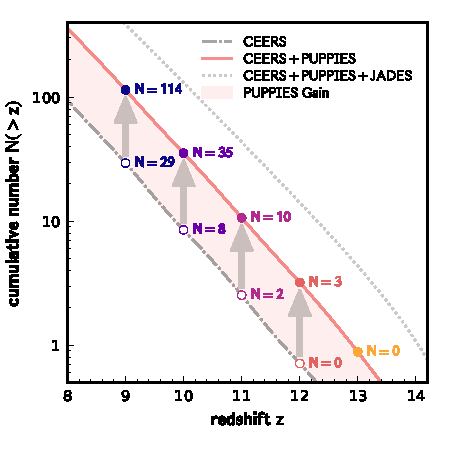
\includegraphics[width=0.49\textwidth]{figs/CN_surveys.pdf}
    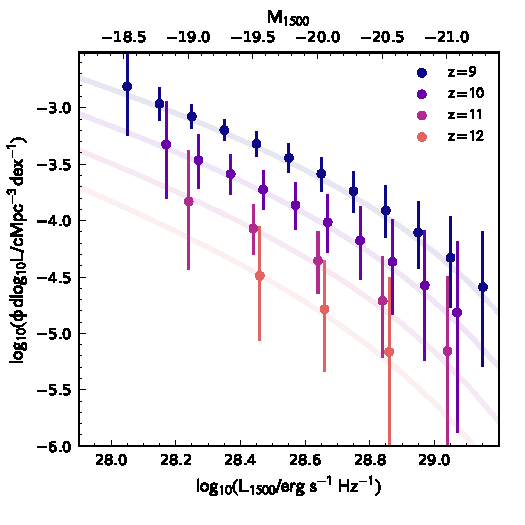
\includegraphics[width=0.49\textwidth]{figs/LF_evo.pdf}
    \vspace{-5mm}
    \caption{\emph{\underline{Left:}} The cumulative number of sources predicted, using predictions from \citet{2019MNRAS.483.2983Y}, observable to CEERS, CEERS+PUPPIES, and CEERS+PUPPIES+JADES.  \emph{\underline{Right:}} Expected constraints on the $z=9-12$ luminosity function from CEERS alone (open symbols) and with PUPPIES. \textbf{PUPPIES will boost the number of galaxies at $z>9$ ($z>11$) by a factor of $4$ (5) compared to CEERS alone yielding much strong constraints on the $z=9-12$ luminosity function.}}
    \label{fig:vs_CEERS}
\end{figure}

PUPPIES will overcome these issues by bridging the gap between CEERS and JADES in cycle 1 by collecting $\sim 150\ {\rm arcmin^2}$ multi-band observation with F200W=$29.2-29.6$. Crucially, unlike the contiguous fields surveyed by CEERS and JADES, PUPPIES will collect data in multiple independent sight lines, significantly reducing the impact of cosmic variance on uncertainties. Using the methodology of \citet{2020MNRAS.499.2401T} we find that, compared to a similar area contiguous survey, the PUPPIES strategy reduces cosmic variance by $3-4\times$ reducing the overall uncertainty by $\sim 2\times$ and leaving it mostly dominated by statistical (Poisson) noise. Fig. \ref{fig:vs_CEERS} demonstrates the improvement to the cumulative number of sources and luminosity functions at $z>9$ with the addition of PUPPIES compared to CEERS alone. PUPPIES will increase the number of accessible $z>9$ ($z>11$) sources by $\sim 4\times$ ($\sim 5\times$) compared to CEERS alone. As demonstrated in Fig. \ref{fig:alpha} this translates to the first meaningful constraints on the faint-end slope $\alpha$ at $z>8$. At $z=9$ we forecast being able to constrain $\alpha$ to $\pm 0.15$. Combined with constraints on the normalisation this is enough to differentiate between many different theoretical models and thus constrain some of the physical processes responsible for the formation of galaxies in the early Universe.




\begin{figure}[h!]
    \centering
    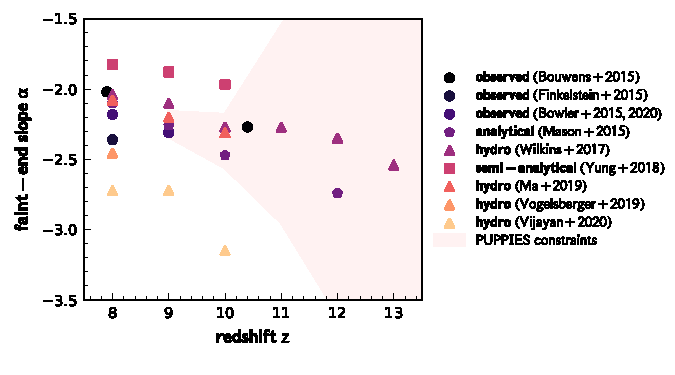
\includegraphics[width=0.8\textwidth]{figs/alpha.pdf}
    \vspace{-5mm}
    \caption{Current observational constraints and theoretical predictions for the faint-end slope $\alpha$ of the luminosity function at $z\ge 8$ alongside forecasts for constraints from PUPPIES + CEERS. \textbf{Predictions for the faint-end slope of the luminosity function $\alpha$ at $z=8-13$ are highly variable. PUPPIES will provide the first meaningful constraints at $z>8$.}}
    \label{fig:alpha}
\end{figure}






\subsection*{\bf \underline{The Physical Properties of the First Galaxies}}

\noindent
\textbf{Early Enrichment with Metals and Dust} - As we look back towards the Big Bang the galaxies we discover become increasingly deficient in metals and dust. Exactly when and how the first galaxies became enriched with metals are key outstanding questions in galaxy formation and evolution.

While accurate measurements of the gas and stellar phase metallicities require deep rest-frame optical spectroscopy we can gain the first hints from photometry alone, specifically from the UV continuum slope $\beta$,  where $f_{\lambda}\propto\lambda^{\beta}$. Extremely blue ($\beta = -3$) slopes are only realised for extremely metal poor and dust free stellar populations. The robust identification of galaxies with such slopes will, for the first time, provide the first glimpse into virtually metal-free stellar populations. More generally the UV continuum slope, at least for young star forming galaxies as expected at $z>9$, is sensitive to dust attenuation, itself a tracer of metal enrichment. Thus, while the discovery of galaxies with extremely blue slopes will be exciting, the discovery of galaxies with $\beta > -2$, indicating the presence of dust, also provides useful observational constraints on the process of metal and dust enrichment in the early Universe \citep[e.g.,][]{2017ApJ...837L..21L}. 

At present, constraints with \emph{Hubble} are effectively limited to $z\sim 7$ (e.g., \citealt{Finkelstein2012, Bouwens2014, Bhatawdekar2020}). Even there $\beta$ is only constrained with a single colour probing only a relatively narrow wavelength range leading to large uncertainties. While it is possible to measure $\beta$ at $9<z<11$ by combining {\em Hubble} and {\em Spitzer} observations \citep[e.g.,][]{2016MNRAS.455..659W} this relies on the significantly shallower, and often confused, {\em Spitzer} imaging resulting in much larger uncertainties. 

With our fiducial 6-band strategy we will be able to, for the first time, \emph{consistently} measure $\beta$'s with high-precision ($\Delta\beta <0.1$) across the entire reionization epoch $6<z<12$. In doing so we will constrain the metal and dust enrichment of galaxies in the early Universe.

\vspace{2mm}
\noindent
\textbf{Stellar populations} - In addition to $\beta$, PUPPIES will also obtain F444W photometry, probing beyond the Balmer-break at $9<z<11$. When combined with a measure of the UV continuum slope $\beta$ this enables - see technical justification - us to measure stellar masses, and thus constrain the galaxy stellar mass function and stellar mass - specific star formation rate relation. With PUPPIES we will measure the galaxy stellar mass function at $z>9$, and where ancillary optical observations are available, at $z<9$. The stellar mass function and specific star formation rate - stellar mass relation provide an additional constraint on the processes responsible for the early formation of galaxies. For example, discovery of objects with suppressed, or quenched, star formation in the early Universe may point to stronger stochastic feedback than currently implemented in models.  

\vspace{2mm}
\noindent
\textbf{Resolved Structures} - The resolved structures of galaxies encode information about their structural properties and formation histories which can be compared to galaxy formation models.  However we know very little concerning the properties of $z > 9$ galaxies, and even basic information like sizes would be revealing  useful physical information.     Structure can also be used in the statistical measurement of the luminosity function, for completeness simulations, and only by simultaneously modelling the structures, redshifts, and fluxes is it possible to self-consistently measure the luminosity function and its uncertainties.   As can be seen in Fig. \ref{fig:sizes} we will be able to determine structural properties of many galaxies.

\begin{wrapfigure}{r}{0.6\textwidth}
\vspace{-5mm}
  \begin{center}
    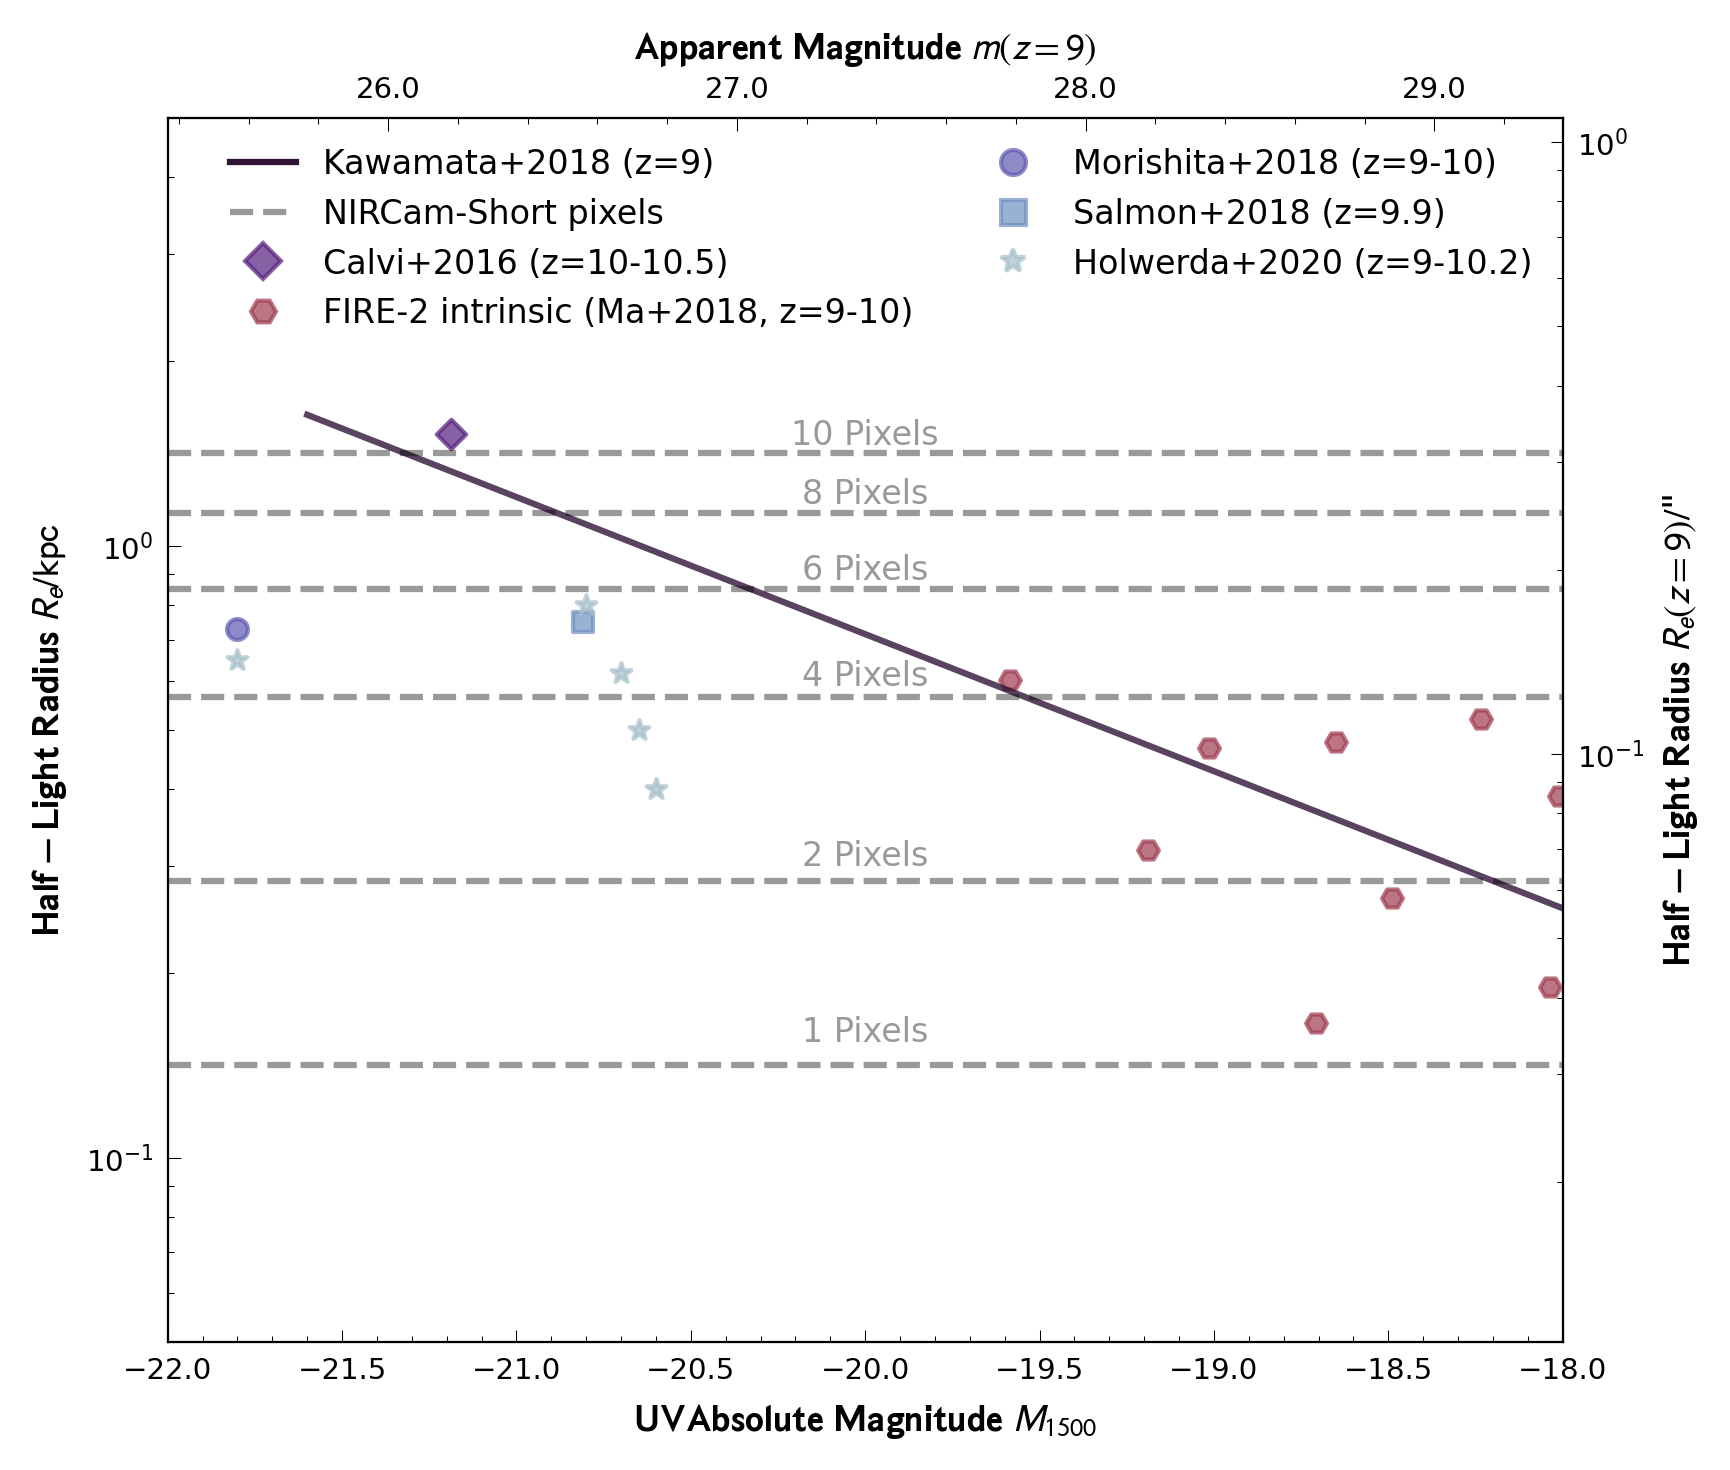
\includegraphics[width=0.95\textwidth]{figs/morph.png}
  \end{center}
  \vspace{-5mm}
  \caption{Current observation constraints and theoretical predictions for the sizes of galaxies at $z>9$. \textbf{Even in under-sampled imaging many $z>9$ galaxies are expected to be resolved in the NIRCam imaging.}}
   \label{fig:sizes}
\end{wrapfigure}

We know that massive galaxies at $z < 6$ are often very compact and evolve into red nuggets that have extinguished their star formation a few Gyr after the big bang.  What we do not know is how this occurred.  These quenched ‘red nuggets’ are up to five times smaller at $z\sim3-6$ than galaxies of the same mass today.  Since these are certainly the progenitors of modern massive galaxies, studying the ancestors of these compact passive/red galaxies at even higher redshifts is crucial for deciphering their origin.   PUPPIES will answer how these early galaxies first formed -- were they large star forming systems that later become compact through some process (e.g., \citealt{Barro2013,Tacchella2016})? Or, did they form as compact systems to begin with (e.g., \citealt{Lilly2016})?   

%Because our parallel imaging will find the most massive systems, and therefore the progenitors of these passive galaxies, we can answer this question by measuring the sizes of these galaxies.

It is clear that merging activity is very important for distant galaxies up to $z \sim 6$ and likely is even more important at higher redshifts.  The evolution of the density of matter at these early phases of the universe goes as $\sim (1+z)^{3}$, such that galaxies at $z > 9$ were in a more dense universe than at later times.  \citet{Duncan2019} showed that $\sim 40$\% of massive galaxies at $z \sim 6$ are in pairs, with an inferred merger rate of $\sim 10$ mergers Gyr$^{-1}$.  In hierarchical models of galaxy formation these galaxies should have undergone intense merging, which is something that we directly detect. It is ideal to test this with massive systems, which would be the easiest to find observational signatures of mergers in, given that the secondary system in a pair can be over a magnitude fainter.  If we extrapolate the merger fraction history that we can measure at $z > 6$ we find that there should be over 60\% of galaxies in pairs at $z > 9$.  This is also a prediction of models such as Illustris and Eagle, which we can test at this high density region of the early universe.  Given that we will detect $\sim 100$ galaxies, our shot noise will produce a merger fraction which is less than 10\% on this measurement.  




\subsection*{\bf \underline{Legacy science}}

With a pure parallel project such as this, there are many additional science topics that can be addressed.  This includes, but is not limited to, faint low-mass stars and sub-stellar objects, quiescent galaxies at lower redshifts, and the morphologies of field galaxies. Some of these goals would require spectroscopy or deep observed optical imaging, but many of them can be achieved just with the \emph{Webb} imaging that we will acquire.

\vspace{2mm}
\noindent
\textbf{Low-mass stars and sub-stellar objects} One of the primary legacy science topics that can be done with PUPPIES using just \emph{Webb} data is to search for low-mass stars and sub-stellar objects (MLTY spectra type). These stars are not only identifiable in the near-IR but are ubiquitous in imaging observations.  Their distribution across the Galaxy is unknown and thus probes such as ours which will locate these stars are ideal for studying these objects as well as their density and distributions. There are currently good statistics in the immediate Solar neighbourhood for stars such as these, they are largely unexplored beyond. Because our observations will probe both the distinct absorption features of later type stars, and the Rayleigh-Jeans slope of their spectra,  PUPPIES will provide an unambiguous type and sub-type for these objects. With multiple independent sight lines, PUPPIES will break the local density/scale-height and scale-length degeneracy of local measurements using these stars.

\vspace{2mm}
\noindent
\textbf{A coherent picture of galaxy assembly across cosmic history} The deep near-IR JWST imaging from PUPPIES will provide an excellent foundation for future spectroscopic studies with the NIRSpec MOS, or NIRCam/NIRISS WFSS. The PUPPIES data will provide a high source density that will make efficient use of these MOS instruments. The efficient near-IR spectroscopy enabled by PUPPIES will not only provide precise redshifts but also provide multi-line metallicities of galaxies at $z=1-4$ down to $M_{*}=10^{8}\ {\rm M_{\odot}}$ and H$\alpha$ based star formation rates. 






%%%%%%%%%%%%%%%%%%%%%%%%%%%%%%%%%%%%%%%%%%%%%%%%%%%%%%%%%%%%%%%%%%%%%%%%%%%

%   2. TECHNICAL JUSTIFICATION
%       (see https://jwst-docs.stsci.edu/jwst-opportunities-and-policies/jwst-call-for-proposals-for-cycle-1/jwst-cycle-1-proposal-preparation)
%
%

\clearpage

\justifyobservations   % Do not delete this command.
% Enter your description of the observations.

In this section we justify our choices of survey parameters including the choice of filters, depth, and area, and assess the potential available pure parallel observing opportunities.

\vspace{2mm}
\noindent
\underline{\bf Filter choice: photometric redshifts -- } High-redshift star forming galaxies can be identified by taking advantage of the strong Lyman-limit/$\alpha$ break combined with the relatively flat continuum beyond. This technique - the Lyman break technique - has been applied numerous times over the last 25 years to successfully identify star forming galaxies to $z\sim 10$. In the simplest implementation of this technique high-redshift galaxies can be isolated in colour (or flux-ratio) space as demonstrated in Fig. \ref{fig:s_f}: the strong break manifests as a very red colour (or small flux ratio) while the continuum has a colour $\sim 1$ (or flux ratio close to unity). The analysis presented in \ref{fig:s_f}, based on synthetic observations from \citet{2018MNRAS.478.1694M}, demonstrated that just 3-bands ({\bf F115W}, {\bf F150W}, and {\bf F277W}) can be used to efficiently identify $z>9$ galaxies with relatively low contamination. However, one disadvantage of this approach is the relatively large scatter $\Delta z/(1+z)>0.1$ in the redshifts of individual galaxies resulting in large  uncertainties on individual luminosities. By adding three additional filters ({\bf F200W}, {\bf F356W}, and {\bf F444W}) it is possible to not only determine much more precise redshifts ($\Delta z/(1+z)<0.05$) but also reduce the contamination rate to $<5\%$. 

\begin{SCfigure}[][!h]
    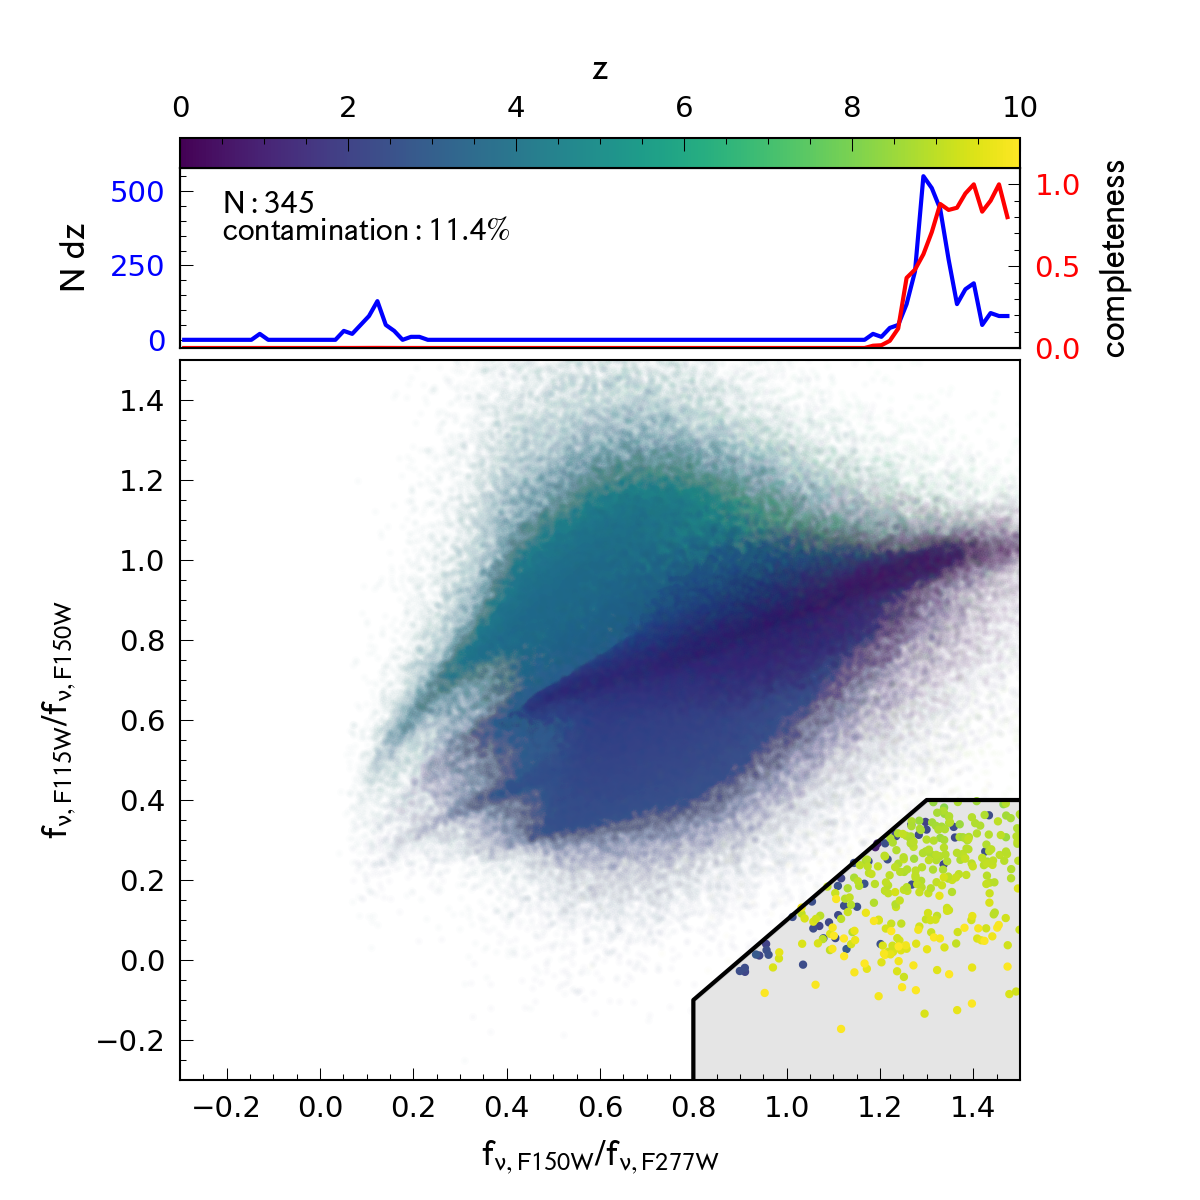
\includegraphics[width=0.6\textwidth]{figs/s_f_F115W.png}
      \caption{\protect\rule{0ex}{10ex} The flux analogue of a colour-colour selection for $9<z<11$ galaxies. Using a mock catalogue from \citet{2018MNRAS.478.1694M} combined with photometric noise consistent with our middle tier we demonstrate that a simple pair of flux ratios (or colours) can be used to efficiently select galaxies at $9<z<11$ with contamination $\sim 10\%$ and high-completeness. Sources are only included if they are detected in F277W$>7\sigma$.}
      \label{fig:s_f}
\end{SCfigure}

\begin{figure}[h!]
    \centering
    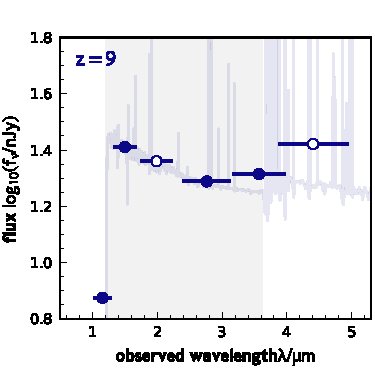
\includegraphics[width=0.3\textwidth]{figs/SED_9.pdf}
    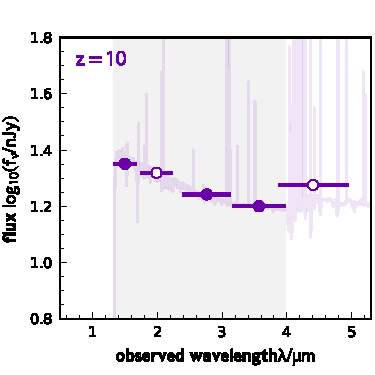
\includegraphics[width=0.3\textwidth]{figs/SED_10.pdf}
    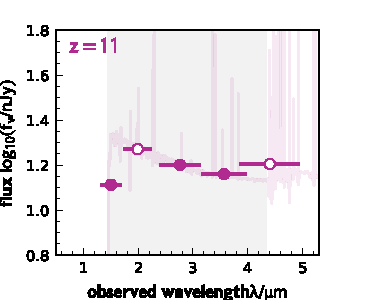
\includegraphics[width=0.3\textwidth]{figs/SED_11.pdf}
    \caption{The model spectral energy distribution and 6-band NIRCam fluxes of a star forming galaxy at $z=9$, $10$, and $11$. The shaded area denotes the rest-frame UV continuum between the Lyman-$\alpha$ and Balmer breaks. The alternative 4-band strategy is denoted by the filled symbols. \textbf{The 6-band PUPPIES strategy allows the consistent measurement of the UV continuum slope across the entire UV continuum and redshift range. An alternative 4-band strategy allows the measurement of the slope albeit only with a single pair of filters. The 6-band strategy additionally allows us to measure a single band beyond the Balmer-break, essential for measuring stellar masses.}}
    \label{fig:SED}
\end{figure}

\noindent
\underline{\bf Filter choice: physical properties -- } Constraining the chemical and dust enrichment of galaxies at $9<z<11$ requires that we probe the rest-frame UV continuum with at least a single colour, and ideally with several bands providing a consistent measurement of the same wavelength range across several redshifts. As demonstrated in Fig. \ref{fig:SED} a 3-pair strategy is ideal in this respect as it allows the UV continuum to probed with 3 bands uncontaminated by the Lyman-$\alpha$ and Balmer breaks, encompassing the entire rest-frame UV, across our entire target redshift range. A 2-pair strategy allows the measurement of the slope albeit with only a pair of filters uncontaminated by the breaks. 

\begin{figure}[h!]
    \centering
    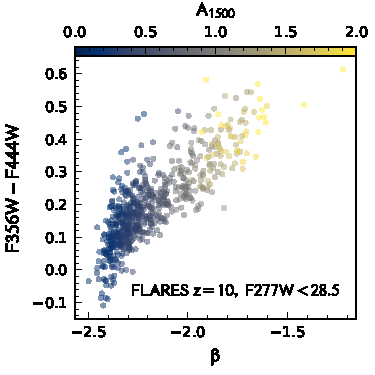
\includegraphics[width=0.45\textwidth]{figs/beta_A1500.pdf}
    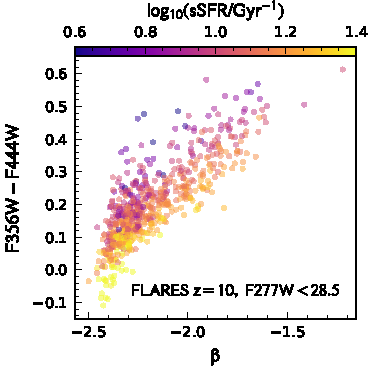
\includegraphics[width=0.45\textwidth]{figs/beta_sSFR.pdf}
    % 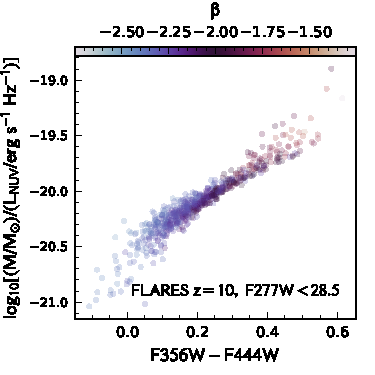
\includegraphics[width=0.3\textwidth]{figs/C_beta_MTOL.pdf}
    \caption{The relationship between $\beta$ and F356W-F444W for simulated galaxies at $z=10$ colour-coded by $A_{1500}$ (\emph{\underline{left}}) and specific star formation rate (\emph{\underline{right}}) predicted by the FLARES simulation (\citealt{2020MNRAS.tmp.3168L, Vijayan2020}). At these redshifts $\beta$ is strongly correlated with dust attenuation while at fixed $\beta$ the specific SFR is correlated with F356W$-$F444W. \textbf{The 6 filter observations obtained by PUPPIES will enable us to measure the dust attenuation, total star formation rates, and stellar masses of galaxies at $z>8$.}}
    \label{fig:beta}
\end{figure}

The strength of the Balmer break, often measured with a broadband colour, is a well established diagnostic of the recent star formation activity in galaxies. However, the broadband break colour is also sensitive to dust attenuation and thus, in the absence of additional constraints, the observed colour is degenerate. However, the UV continuum slope $\beta$ is a well established diagnostic of dust attenuation: redder galaxies are generally dustier. Combining these two diagnostics then allows us to constrain both the dust attenuation and the specific star formation rate. This is demonstrated in  Fig. \ref{fig:beta} where simulated galaxies, from the FLARES project \citep{2020MNRAS.tmp.3168L}, are shown in the $\beta$ and F356W-F444W plane and colour coded by $A_{1500}$ (left) and specific star formation rate (right). At fixed $\beta$ F356W-F444W is correlated with specific star formation rate. Measuring both $\beta$ and F356W-F444W then allows us to constrain the specific star formation rate and stellar mass. A 3-pair strategy allows us to include {\bf F444W} providing access to the spectrum beyond the Balmer break.

\vspace{2mm}
\noindent
\underline{\bf Filter choice: alternative strategies -- } While a 3 filter pair strategy best matches our full scientific objectives, our core objective - meaningful constraints on the faint-end of the luminosity function - can be achieved with a 2-pair strategy. To allow PUPPIES to efficiently use the maximum number of opportunities, while still fulfilling our core objective, we can also make use of opportunities better suited to a 2-pair strategy.

\vspace{2mm}
\noindent
\underline{\bf Area and Depth - } In the absence of cosmic variance, the core science objective of PUPPIES - to constrain the faint-end slope and normalisation of the $9<z<11$ UV luminosity function - is best realised by going as deep as possible. This is both because the expected number of galaxies increases faster than $f_{\nu}^2$ due to the steepness of the luminosity function and going deeper extends the luminosity range. Going deeper also provides stronger complementarity with the public $\sim 90\ {\rm arcmin}^2$ CEERS NIRCam imaging. However, a single, or small number of fields, is susceptible to cosmic-variance, which will dominate over the statistical (Poisson) variance \citep[e.g.,][]{2020MNRAS.499.2401T}. From our analysis, based on the methodology of \citet{2020MNRAS.499.2401T}, a good compromise is afforded by combining $10-20$ pointings with durations $10^4-10^5$s long yielding depths of F200W=$29-30$. This provides an area comparable to CEERS (and thereby doubling the available public imaging) but will reach up-to $1$ magnitude deeper.


\vspace{2mm}
\noindent
\underline{\bf Availability of deep NIRCam parallel opportunities - }
To determine the type, and thus potential depth, of opportunities that are available we use the public GTO and ERS APTs and filter out all observations that 1) already have attached coordinated parallels, 2) have the \texttt{NoParallel} flag set, and 3) are targets with high-background ($>0.3\ {\rm MJy/Sr}$). To estimate the amount of time available to each unique target we sum the science durations of all observations using the same instrument. The predicted distribution of opportunities with science durations $t_{\rm SD}>10^{4}$ s is then shown in Figure \ref{fig:time_background}: this analysis suggests $\sim 50$ GTO/ERS opportunities with $t_{\rm SD}>10^{4}$ s; assuming this distribution is representative of the final Cycle 1 observations suggests there should be $100-150$ useful opportunities.

\begin{SCfigure}
    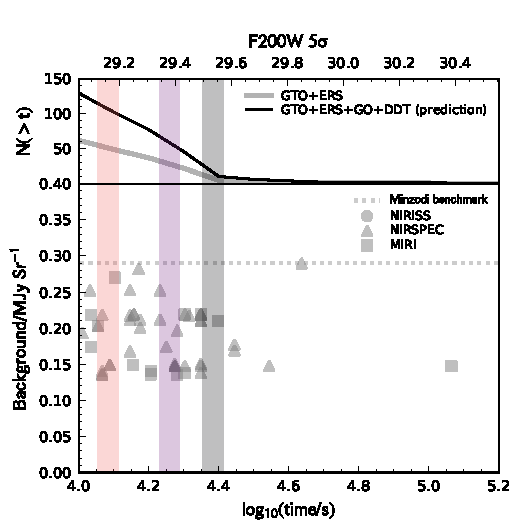
\includegraphics[width=0.6\textwidth]{figs/time_background.pdf}
      \caption{\protect\rule{0ex}{10ex} The predicted distribution of science durations $t_{\rm SD}$ and backgrounds for pure parallel observing opportunities based on the existing GTO and ERS programs. The vertical bands denote the 3 tiers used to define our fiducial survey while the horizontal lines denote the $2\mu$m \texttt{minzodi} benchmark background and the minimum background in several deep extragalactic fields. The top panel shows the resulting cumulative distribution of opportunities as well as an extrapolation to the full cycle 1 observations.}
      \label{fig:time_background}
\end{SCfigure}

\vspace{2mm}
\noindent
\underline{\bf Fiducial programme:} Armed with this knowledge of the predicted number and distribution of available parallel opportunities we define a fiducial programme consisting of three tiers - ABC - assuming 4, 3, and 2 \texttt{deep8} 10 group exposures respectively. Reflecting the greater availability of shorter duration opportunities we choose, for this fiducial programme, to obtain 3, 5, and 10 pointings for the A, B, and C tiers respectively. The resulting area and depths achieved in each tier are summarised below. Our shallowest tier (C) covers an area similar to CEERS but is $\sim 0.2$ mag deeper (in F200W) - see Fig. \ref{fig:F200W}. \textbf{The total exposure time as reported by the APT for the combination of the 3 tiers is 79.3 hours}. This fiducial programme serves only to demonstrate what should be possible with a PUPPIES-\emph{like} programme and not a firm requirement.

\begin{table}[h!]
\footnotesize
\begin{center}
\begin{tabular}{ |c|c|c|c|c|c|c|c|c| } 
\hline
\multicolumn{3}{|c|}{} & \multicolumn{6}{|c|}{$5\sigma$ point-source depth} \\
 \hline
Tier & $N_{p}$ & Area$/{\rm arcmin^2}$ & F115W & F150W & F200W & F277W & F356W & F444W \\
\hline
\textbf{A} & 3 & 27 & 29.19 & 29.37 & 29.54 & 29.09 & 29.15 & 28.86 \\
\textbf{B} & 5 & 45 & 29.03 & 29.22 & 29.38 & 28.94 & 28.99 & 28.70 \\
\textbf{C} & 10 & 91 & 28.81 & 28.99 & 29.16 & 28.71 & 28.77 & 28.48 \\
\hline
\end{tabular}
\end{center}
\vspace{-5mm}
\caption{The number of pointings $N_p$, area, and 5$\sigma$ point source depths in each filter for our 3 tiers for our fiducial survey.  Depths assume a short-wavelength (long-wavelength) apertures of $0.08$" ($0.16$"), background at the benchmark level of the \texttt{Minzodi} location as defined by \texttt{Pandeia}. The ABC tiers assume 4, 3, 2 exposures of 10 groups assuming the \texttt{DEEP8} readout mode respectively.}
\end{table}

\begin{SCfigure}[][!h]
    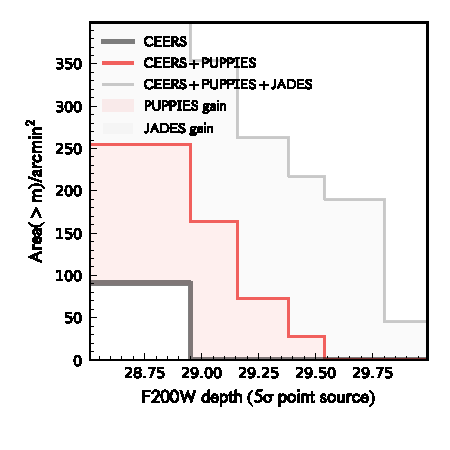
\includegraphics[width=0.45\textwidth]{figs/F200W.pdf}
  \caption{\protect\rule{0ex}{10ex} The cumulative area probed by the fiducial PUPPIES program, JADES, and CEERS, as a function of the F200W depth. \textbf{PUPPIES will more than double the area of public deep NIRCam imaging while also pushing $0.2-0.6$ mag deeper.}}
  \vspace{-5mm}
  \label{fig:F200W}
\end{SCfigure}




\vspace{2mm}
\noindent
\underline{\bf Preferred distribution and flexibility - } The fiducial programme defined above serves only to demonstrate what should be possible with a PUPPIES-\emph{like} programme and is not a firm requirement. Within the confines of our requirement for 10-20 deep (F200W$>29$), low-background, independent pointings we are flexible in our choice of observing opportunities. We will however seek to obtain a balanced programme mixing deeper and shallower opportunities. Where possible we will also express a preference for targets with meaningful existing observations and ones that are accessible to the Southern Hemisphere.

\vspace{2mm}
\noindent
\underline{\bf Treasury Data Plan - } While focused on the distant Universe the PUPPIES data-set will have tremendous legacy value to the community allowing multiple scientific questions in both galactic and extragalactic astronomy to be answered. To facilitate the exploitation of PUPPIES we will release several high-level data products including reduced images, photometry catalogues, and catalogues containing redshifts and physical properties derived from SED fitting. We will also make many of our analysis scripts publicly available. 
Depending on scheduling some of PUPPIES observations may be available before the cycle 2 call deadline. Where this is the case we will endeavour to release at least basic data-products as soon as possible to enable members of the community to utilise these for cycle 2 proposals. For example, many of the fields would be excellent sources of targets for NIRSpec MOS.








%%%%%%%%%%%%%%%%%%%%%%%%%%%%%%%%%%%%%%%%%%%%%%%%%%%%%%%%%%%%%%%%%%%%%%%%%%%

%   3. SPECIAL REQUIREMENTS
%        (see https://jwst-docs.stsci.edu/jwst-opportunities-and-policies/jwst-call-for-proposals-for-cycle-1/jwst-cycle-1-proposal-preparation)
%
%
\specialreq             % Do not delete this command.
% Justify your special requirements here, if any.

%%%%%%%%%%%%%%%%%%%%%%%%%%%%%%%%%%%%%%%%%%%%%%%%%%%%%%%%%%%%%%%%%%%%%%%%%%%

%   4. COORDINATED PARALLEL OBSERVATIONS
%        (see https://jwst-docs.stsci.edu/jwst-opportunities-and-policies/jwst-call-for-proposals-for-cycle-1/jwst-cycle-1-proposal-preparation)
%
%
\vspace{-5mm}
\coordinatedobs % Do not delete this command.
% Enter your coordinated parallel observing plans here, if any.

%%%%%%%%%%%%%%%%%%%%%%%%%%%%%%%%%%%%%%%%%%%%%%%%%%%%%%%%%%%%%%%%%%%%%%%%%%%

%   5. JUSTIFY DUPLICATIONS
%        (see https://jwst-docs.stsci.edu/jwst-opportunities-and-policies/jwst-call-for-proposals-for-cycle-1/jwst-cycle-1-proposal-preparation)
%
%
\vspace{-5mm}
\duplications           % Do not delete this command.
% Enter your duplication justifications here, if any.

%%%%%%%%%%%%%%%%%%%%%%%%%%%%%%%%%%%%%%%%%%%%%%%%%%%%%%%%%%%%%%%%%%%%%%%%%%%

%   6. ANALYSIS PLAN
%       (see https://jwst-docs.stsci.edu/jwst-opportunities-and-policies/jwst-call-for-proposals-for-cycle-1/jwst-cycle-1-proposal-preparation)
%
%
\vspace{-5mm}
\analysisplan % Do not delete this command.
% Describe the data processing and analysis plan here.

%%%%%%%%%%%%%%%%%%%%%%%%%%%%%%%%%%%%%%%%%%%%%%%%%%%%%%%%%%%%%%%%%%%%%%%%%%%

\clearpage

\bibliography{PUPPIES.bib}


\end{document}          % End of proposal. Do not delete this line.
                        % Everything after this command is ignored.
